%!TEX root = ../main.tex

%----------------------------------------------------------------------------%
\subsubsection{Mass Model}
\label{sec:b02dd:systematics:massmodel}

Two different aspects of the mass model are studied regarding systematic
uncertainties: the impact of neglecting contributions and of mismodelling
components.

\paragraph{Neglected contributions}

If a neutral \piz or a photon is missed in the reconstruction the decay
\BToDstD, with \DstpToDpizero or \DstpToDgamma, can mimic the \BToDD decay. In
the rest frame of the \Dstarp resonance, the missing momentum of the \piz is
fixed, but it needs to be boosted when transferred into the rest frame of the
\PB meson. So, the reconstructed mass depends on the helicity angle of the
missing \piz. This leads to a double-horned structure approximately
\SI{140}{\MeVcc} below the nominal \PB mass (see Ref.~\cite{LHCb-ANA-2014-015}
for more details on the shape of this background). As the lower boundary on
the invariant $m_{\Dp\Dm}$ mass is set to \SI{5150}{\MeVcc} the \BdToDstD
contribution lies outside the mass range used for the fit. However, the
\BsToDstD contribution enters the fit region. But since the expected number of
\BsToDstD candidates is low, it is not included in the nominal mass model.
Another contribution that is neglected in the nominal mass fit model is
(partially) charmless background where at least one of the hadron triplets is
not originating from a \PD decay. The systematic uncertainty on the
determination of the \CP observables arising from neglecting these two
contributions is estimated using \num{1000} pseudoexperiments. Components for
\BsToDstD and for (partially) charmless background are included in the
generation but excluded from the fit procedure.

The shape of \BsToDstD is parametrised with two single Gaussian functions
centred around \SI{5150}{\MeVcc} and \SI{5200}{\MeVcc}. The (partially)
charmless background is modelled with a single Gaussian function. When
optimising the decay time significance cut it has been observed that the width
of the (partially) charmless background is approximately \SI{10}{\percent}
wider than the signal component. Therefore, a width of \SI{10}{\MeVcc} is
chosen. The mean is set to the same position as the \Bd signal. The \BsToDstD
component is generated without any tagging asymmetry, while for the (partially)
charmless background the worst case scenario of maximal \CP violation with the
opposite \CP eigenvalue ($S_f = \num{+1.0}$) is tested.

In studies of \BdToDstD decays~\cite{BToDstDthesis} a significant contribution
of \BsToDstD candidates is observed. The ratio between the two yields is
determined to be 1:20. Under the assumption that the efficiencies for \BToDD
and \BToDstD are the same the expected number of \BsToDstD candidates can be
calculated via
\begin{align}
	\text{N}_{\BsToDstD} = \frac{1}{20} \text{N}_{\BdToDD} \frac{\mathcal{B}(\BdToDstD) \mathcal{B}(\Dstarp \!\to \Dp (\piz || \gamma))}{\mathcal{B}(\BdToDD)} \,.
\end{align}
Using the world averages for the branching ratios~\cite{PDG2016} the number of
candidates to be generated in the pseudoexperiments is estimated to be
N(\BsToDstD) = \num{66\pm9}.

To determine how many (partially) charmless background candidates need to be
generated the $D$ mass window is widened to $\SI{\pm40}{\MeVcc}$ and the
nominal $D$ mass window of $\SI{\pm25}{\MeVcc}$ is vetoed for one or for both
$D$ candidates. Fits to the invariant $B$ mass without the $D$ mass constraint
are performed in the various scenarios. % yielding
% $\num{0.0\pm2.6}\,\mbox{\Bd\!\to\KpipiKpipi}$ candidates,
% $\num{0.0\pm9.2}\,\mbox{\Bd\!\to\KKpiKpipi}$ candidates,
% $\num{0.0\pm4.9}\,\mbox{\Bd\!\to\D(\Kpipi)\Kpipi}$ candidates,
% $\num{0.0\pm3.3}\,\mbox{\Bd\!\to\D(\KKpi)\Kpipi}$ candidates, and
% $\num{17.2\pm11.2}\,\mbox{\Bd\!\to\D(\Kpipi)\KKpi}$ candidates.
%
The fitted yields, which are constrained to positive values, are scaled to
account for the applied $D$ mass window. The total amount of residual
contamination ($\Bz\!\to\PD hhh$ or $\Bz\!\to hhhhhh$ decays) surviving the
\BdToDD selection is found to be $\num{28.7\pm19.5}$ candidates for the
$\KKpiKpipi$ final state and $\num{0.0\pm27.8}$ candidates for the
$\KpipiKpipi$ final state. For the pseudoexperiments the number of (partially)
charmless background is drawn from Gaussian distributions using these values
for mean and width. When the outcome is negative the procedure is repeated,
until a positive yield is drawn.

The systematic uncertainties on \SDD and \CDD are calculated as the product of
the bias on the mean parameter of the pull distributions and the statistical
uncertainty:
\begin{align*}
s_{\SDD}^{\text{mass,1}} = \num{0.05}\ , \qquad s_{\CDD}^{\text{mass,1}} = \num{0.013}\,.
\end{align*}

\paragraph{Mismodelling of mass components}

The BDT is trained with MC samples that are known to not perfectly model the
PID information. As a result the BDT classifier distributions of
background-subtracted data and MC show a quite big discrepancy. Some shape
parameters are estimated on MC samples and might be distorted by the data/MC
differences. Therefore, different alternative mass parametrisations are tested
against the nominal model: the component of the \BdToDD signal (and of the
\BsToDD background) is parametrised with a single Gaussian function; the
combinatorial background is described with a second order Chebyshev polynomial
of first kind; the tail parameters of \BToDsD are once extracted from the MC
sample without applying the BDT and once applying a tight cut on the BDT
classifier. The mass fit is performed with these new models, sWeights are
calculated for each approach, and the decay time fit is performed. The results
of the \CP observables are then compared with the nominal central values. The
largest deviations for \SDD and \CDD are
\begin{align*}
s_{\SDD}^{\text{mass,2}} = \num{0.004}\ , \qquad s_{\CDD}^{\text{mass,2}} = \num{0.006}\,.
\end{align*}

%----------------------------------------------------------------------------%
\subsubsection{Correlation between decay time and mistags}
\label{sec:b02dd:systematics:correlation_mistag_time}

The correlation between the decay time distribution and the per-event mistags
is studied by calculating the linear Pearson correlation coefficient
$\rho(\eta,t)$. The significance of the correlation value, \ie
\SI{95}{\percent} confidence level interval, is determined using the
bootstrapping method (\cref{sec:dataanalysis:bootstrapping}) with \num{10000}
repetitions. The correlation coefficients are found to be small. The profile
histogram of the OS tagging combination, which shows the average \etaos value
as a function of the decay time, is flat within statistics. For the SS tagging
combination the profile histogram slowly increases with decay time. This can
be confirmed by analysing the larger signal MC sample (see
\cref{fig:b02dd:systematics:correlation_mistag_time:etass_time_profile_MC}).
\begin{figure}[htb]
\centering
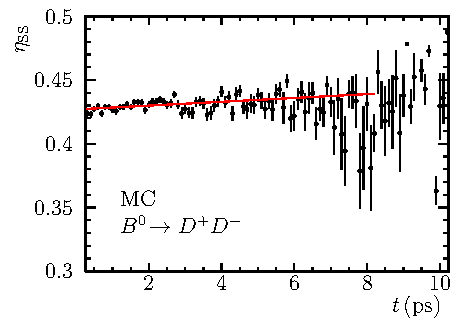
\includegraphics[width=0.6\textwidth]{07-B02DD/tikz/pdf/Profile_DecayTime_SS.pdf}
\caption{Profile histogram for the decay time dependence on $\etass$ for
signal MC. The black data points represent the mean value of $\etass$ and its
uncertainty for each bin in $t$. The red curve is the fitted linear function.}
\label{fig:b02dd:systematics:correlation_mistag_time:etass_time_profile_MC}
\end{figure}
Performing a $\chisq$ fit in the decay time range \SIrange{0.25}{8.25}{\ps}
with the linear function
\begin{align}
  \etass = a_{\etass,t} t + b_{\etass,t}
  \label{eq:tagging:correlation_mistag_time}
\end{align}
yields a slope of $a_{\etass,t} = \SI{1.50\pm0.27}{\invns}$. Although this is
a significant deviation from zero, the correlation is not taken into account in
the nominal fit model. Instead, a study on the systematic uncertainty from
neglecting this effect is performed. In \num{1000} pseudoexperiments the SS
mistag is generated using a Gaussian distribution whose mean is drawn from the
linear function defined in \cref{eq:tagging:correlation_mistag_time} thereby
introducing the correlation with the decay time. In the subsequent fit the
correlation is again ignored. This leads to systematic uncertainties of
\begin{align*}
s_{\SDD}^{\text{corr}} = \num{0.0007}\ , \qquad s_{\CDD}^{\text{corr}} = \num{0.007}\,.
\end{align*}

%----------------------------------------------------------------------------%
\subsubsection{Decay Time Resolution Model}
\label{sec:systematics:decaytimeresolution}

As calculated in \cref{sec:b02dd:decaytimefit:resolution} even an
underestimation of the decay time resolution by \SI{15}{\percent} has only a
minor effect on the resolution related dilution. Nevertheless, \num{1000}
pseudoexperiments are performed, in which the scale factors and the offset
parameters ($b_i$ and $c_i$ from \cref{tab:b02dd:decaytimefit:resolution}) are
enlarged by \SI{15}{\percent} in the generation and fixed to their nominal
values in the fit. Additionally, the mean parameter of the Gaussians is set to
the value obtained in the MC study for the generation and, like in the nominal
setup, fixed to zero in the fit. The systematic uncertainties are calculated
as the product of the biases on the mean parameter and the statistical
uncertainty to be
\begin{align*}
s_{\SDD}^{\text{res}} = \num{0.0020}\ , \qquad s_{\CDD}^{\text{res}} = \num{0.0023}\,.
\end{align*}

%----------------------------------------------------------------------------%
\subsubsection{Decay Time Acceptance Model}
\label{sec:systematics:decaytimeacceptance}

On signal MC the decay time acceptance is determined separately for the two
final states (see \cref{fig:b02dd:decaytimefit:acceptance_MC}). Small
differences are observed. As the low statistics in the \KKpiKpipi final state
on data does not allow for an individual spline model, a study is performed to
estimate a possible systematic uncertainty from neglecting this difference. In
\num{1000} pseudoexperiments the decay time distribution is generated using
the histograms of the true decay time acceptance from signal MC, split by
final state, and fitted with the spline acceptance as done in the nominal fit.
The use of the histograms with \num{100} bins should also cover uncertainties
from the choice of the number and position of the knots. The pull between the
fit results and the generation values is calculated. The systematic
uncertainty due to the decay time acceptance model is calculated as the
product of the shift in the pull distribution and the statistical uncertainty
of the nominal fit:
\begin{align*}
s_{\SDD}^{\textrm{acc}} = \num{0.007}\ , \qquad s_{\CDD}^{\textrm{acc}} = \num{0.0027}\,.
\end{align*}
